\section{Ordinary Least Squares and its Application in Statistics}
\subsection{The Orthogonal Decomposition Theorem  and Least-Squares Solution}

\begin{Thm}\label{7-1}
\textbf{The Orthogonal Decomposition Theorem}:
Let $W$ be a subspace of $\mathbb{R}^n$. Then, each $\mathbf{y}$ in $\mathbb{R}^n$ can be written \textbf{uniquely} in the form
\begin{equation}
    \mathbf{y} = \hat{\mathbf{y}} + \mathbf{z}
\end{equation}
where $\hat{\mathbf{y}}$ is in $W$ and $\mathbf{z}$ is in $W^{\bot}$. In fact, if $\{\mathbf{u}_1, \mathbf{u}_2, \cdots, \mathbf{u}_p \}$ is any \textit{orthogonal basis} of $W$, then
\begin{equation}
    \hat{\mathbf{y}} = \cfrac{\mathbf{y}^{\top}\mathbf{u}_1}{\mathbf{u}_1^{\top} \mathbf{u}_1} + \cfrac{\mathbf{y}^{\top}\mathbf{u}_2}{\mathbf{u}_2^{\top} \mathbf{u}_2} + \cdots + \cfrac{\mathbf{y}^{\top}\mathbf{u}_p}{\mathbf{u}_p^{\top} \mathbf{u}_p}
\end{equation}
and $\mathbf{z} = \mathbf{y} - \hat{\mathbf{y}}$.
\end{Thm}

\begin{Def}\label{def-lse}
If $X$ is $n \times p$ and $\pmb{\beta}$ is in $\mathbb{R}^p$, a \textbf{least-squares solution} of of $X\pmb{\beta} = \mathbf{y}$ is an $\hat{\pmb{\beta}}$ in $\mathbb{R}^p$ such that
\begin{equation} \label{LSS}
    \forall \pmb{\beta} \in \mathbb{R}^p: \lVert \mathbf{y} - X\hat{\pmb{\beta}} \rVert \leq \lVert \mathbf{y} - X{\pmb{\beta}} \rVert
\end{equation}
\end{Def}
\noindent We cannot ensure that the linear system $X\pmb{\beta} = \mathbf{y}$ is always consistent. That is, $\mathbf{y}$ may not be in $\text{Col}(X)$. But we can find a $\hat{\pmb{\beta}} \in \mathbb{R}^p$ such that \cref{LSS} holds. Let $\hat{\mathbf{y}} = X\hat{\pmb{\beta}}$, by \textbf{Orthogonal Decomposition Theorem} $\mathbf{y} - \hat{\mathbf{y}}$ is orthogonal to $\text{Col}(X)$, this is,
\begin{equation*}
    \forall i\in \{1, 2, \cdots, p\}: \mathbf{x}_i^{\top} (\mathbf{y} - \hat{\mathbf{y}}) = 0
\end{equation*}
and thus,
\begin{equation*}
    X^{\top}(\mathbf{y} - \hat{\mathbf{y}}) = \mathbf{0} \Longrightarrow X^{\top}  (\mathbf{y} - X\hat{\pmb{\beta}}) = \mathbf{0}
\end{equation*}
We can find $\hat{\pmb{\beta}}$ by solving the following linear system, which is called \textbf{normal equation} and must be consistent
\begin{equation}
    X^{\top}\mathbf{y} = X^{\top}X\hat{\pmb{\beta}}
\end{equation}
Furthermore, if $(X^{\top}X)^{-1}$ exists,
\begin{equation} \label{beta-estimator}
    \hat{\pmb{\beta}} = (X^{\top}X)^{-1}X^{\top}\mathbf{y}
\end{equation}
The same result can be derived from \cref{12 - 1}, using vector calculus.
The prediction vector $\hat{\mathbf{y}}$ (the projection of $\mathbf{y}$ onto $\text{Col}(X)$) can thus be expressed as
\begin{equation}\label{y-estimator}
    \hat{\mathbf{y}} = X(X^{\top}X)^{-1}X^{\top}\mathbf{y} = X\hat{\pmb{\beta}}
\end{equation}
\begin{figure}[ht]
    \centering
    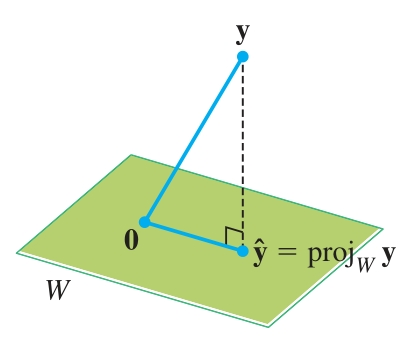
\includegraphics[width=0.25\textwidth]{images/projection-col.jpg}
    \caption{$\Hat{\B{y}}$ is the projection of $\mathbf{y}$ onto $W$, where $W$ is the column space of $\B{X}$.}
   %\label{Find the principal axes.}
    \end{figure}
\begin{Rem}
    In linear model, we are interested in the difference of the response vector $\mathbf{y}$ and its projection onto the column space of design matrix $X$. The \textbf{Sum of Squares due error} is a measurement for that purpose, which is defined as:
    \begin{equation} \label{SSE}
        \text{SSE}(\mathbf{y}) = \lVert \mathbf{y} - X\hat{\pmb{\beta}} \rVert^2 = \sum_{i = 1}^{n} (y_i - \mathbf{x}_i^{\top}\hat{\pmb{\beta}})^2
    \end{equation}
\end{Rem}

\subsection{Orthogonal Projection Matrix}
    By \cref{y-estimator}, we can see that the effect of 
    $X(X^{\top}X)^{-1}X^{\top}$ is to project $\B{y}$ onto $\text{Col}(X)$, which is why it is called \textbf{(Orthogonal) Projection Matrix}. The projection matrix is also called \textbf{Hat Matrix} in statistics. The hat matrix differs from \cref{inner product}, which projects a vector onto a vector, \textbf{while the hat matrix projects a vector onto the column space of $X$}.

\begin{Rem}
    The hat matrix is typically denoted by $H$, it has the following properties:
    \begin{enumerate}
        \item $H$ is symmetric and thus a square matrix.
        \item $H^2 = H$.
        \item If $\mathbf{x}\in\text{Col}(X)$, $H\mathbf{x} = \mathbf{x}$.
    \end{enumerate}
\end{Rem}

\begin{Def}
    \textbf{Idempotent Matrix:} A square matrix $A$ is said to be idempotent if and only if $A^2 = A$.
\end{Def}

\begin{Def}
    \textbf{Orthogonal Projection Matrix}: A matrix $P$ is an orthogonal projection matrix if $P$ is \textbf{idempotent and symmetric}.
    \begin{Rem}
    For any vector $\B{y}$, $P$ projects $\B{y}$ onto a subspace $W$, resulting in $\Hat{\B{y}} = P\B{y}$. If we project $\Hat{\B{y}}$ onto $W$ again, the equation
    \begin{equation}
        \Hat{\B{y}} = P\Hat{\B{y}} = PP\B{y} = P^2\B{y}
    \end{equation} illustrated why $P$ is needed to be \textbf{\textcolor{cyan}{idempotent}}. Conversely, suppose we want to project a vector $\B{y}$ onto a subspace $W$ spanned by $\mathcal{B} = \{\B{v}_1, \B{v}_2,\cdots, \B{v}_n \}$, we can find an orthonormal base by Gram-Schmidt Process, say $\mathcal{U} = \{\B{u}_1, \B{u}_2, \cdots, \B{u}_n\}$. By \cref{orthonormal-projection}, 
    \begin{equation*}
        \hat{\B{y}} = U\T{U}\B{y}
    \end{equation*}
    If we let $P = U\T{U}$, $P$ is clearly \textbf{\textcolor{cyan}{symmetric}}. Note also that \textbf{\textcolor{orange}{$P$ projects a vector onto the subspace spanned by the columns (or rows, since $P$ is symmetric) of $P$}}.
    \end{Rem}
\end{Def}
    We have already known that the hat matrix $H$ is the orthogonal projection matrix onto the column space of $X$, and the residual vector
    \begin{equation*}
        \hat{\epsv} = (\B{y} - H\B{y}) = (I - H)\B{y}
    \end{equation*}
    is orthogonal to $\text{Col}(X)$. It is intuitive to say that $I - H$ is the orthogonal projection matrix onto $\text{Col}(X)^\perp$ or $\text{Nul}(\T{X})$. 
    \begin{Thm}
        If $P$ is an orthogonal projection matrix, then $I - P$ is an orthogonal projection matrix onto $\text{Col}(P)^\perp$ (or $\text{Row}(P)^\perp$, since $P$ is symmetric.
    \end{Thm}
    \begin{Thm}\label{0-1-eigen}
        The eigenvalues of an orthogonal projection matrix $P$  are either $1$'s or $0$'s.
        \begin{proof}
            Since $\forall\mathbf{x}\in\text{Col}(P)$: $H\mathbf{x} = \mathbf{x}$, $\text{Col}(P)$ is an eigenspace of $P$ corresponding to the eigenvalue $1$. And $\forall \B{v}\in \text{Col}(P)^\perp: P\B{v} = 0\cdot \B{v}$ says that $\text{Col}(P)^\perp$ is another eigenspace of $P$ corresponding to eigenvalue $0$. $P$ is a $n\times n$ symmetric matrix, and $\text{dim}\Big(\text{Col}(P)\Big) + \text{dim}\Big(\text{Col}(P)^\perp\Big) = n$, so by \cref{spectral-theorem} $H$ can only have eigenvalues of $0$ or $1$.
        \end{proof}
    \end{Thm}
    \begin{Thm}
        An orthogonal projection matrix is semi-positive definite.
        \begin{proof}
            By \cref{0-1-eigen} and \cref{11-2}.
         \end{proof}
    \end{Thm}

    \begin{Ex}
        Let a quadratic form $Q(\B{x}) = \T{\B{x}}(I - H_0)\B{x}$, where $H_0$ is the projection matrix onto $\mathbbold{1}$ as discussed in \cref{H-0}. Given a vector, what does $Q(\B{x})$ stand for?
        \begin{align*}
            Q(\B{x}) &= \T{\B{x}}(I - H_0)\B{x}\\
            & = \norm{\B{x}}^2 - \T{\B{x}}H_0 \B{x}\\
            & = \norm{\B{x}}^2 - \T{\B{x}}\bar{x}\mathbbold{1}\\
            & = \norm{\B{x}}^2 - \bar{x}\sum_{i = 1}^n x_i\\
            & = \norm{\B{x}}^2 - n\bar{x}^2\\
            & = \sum_{i = 1}^n (x_i - \bar{x})^2 = (n - 1) S^2
        \end{align*}
        where $S^2$ is the sample variance.
    \end{Ex}
\subsection{Application in Linear Model}

    We have calculated $SST$ by \cref{SST}, and we want to calculate the projection vector of $\mathbf{y} - H_0\mathbf{y}$ onto $\text{Col}(X)$
    \begin{equation*}
        H(\mathbf{y} - H_0\mathbf{y}) = H\mathbf{y} - HH_0\mathbf{y} = X\hat{\pmb{\beta}} - \overline{\mathbf{y}}\ \mathbbold{1}
    \end{equation*}
    where $H\mathbf{y}$ is the prediction vector by \cref{y-estimator} and $HH_0\mathbf{y} = H_0\mathbf{y}$ since $H_0\mathbf{y}$ is in $\text{Col}(X)$.
    That is so-called \textbf{Sum of Squares due to Regression}, which is defined as:
    \begin{equation} \label{SSR}
        \text{SSR}(\mathbf{y}) = \lVert X\hat{\pmb{\beta}} - \overline{y}\ \mathbbold{1} \rVert^2 = \sum_{i = 1}^n (\mathbf{x}_i^{\top}\hat{\pmb{\beta}} - \overline{y})^2
    \end{equation}
\begin{Thm}
    We have calculated $SST$, $SSR$ and $SSE$, there is a relationship between them:
    \begin{equation}
        \text{SST}(\mathbf{y}) = \text{SSR}(\mathbf{y}) + \text{SSE}(\mathbf{y})
    \end{equation}
    Or equivalently,
    \begin{equation}\label{7-10}
        \lVert \mathbf{y} - \overline{y}\ \mathbbold{1} \rVert^2 = \lVert X\hat{\pmb{\beta}} - \overline{y}\ \mathbbold{1} \rVert^2 + \lVert \mathbf{y} - X\hat{\pmb{\beta}} \rVert^2
    \end{equation}

    \begin{proof}
        It can be proved by Pythagorean Theorem as shown in \cref{SST-SSE-SSR}.
    \end{proof}
\end{Thm}
\begin{figure}
    \centering
    \begin{tikzpicture}[x=0.75pt,y=0.75pt,yscale=-1,xscale=1]
%uncomment if require: \path (0,300); %set diagram left start at 0, and has height of 300

%Shape: Parallelogram [id:dp8573879965454236] 
\draw   (200.5,117) -- (437.33,117) -- (335.83,213) -- (99,213) -- cycle ;
%Straight Lines [id:da6339390874989326] 
\draw    (200.5,117) -- (274.3,89.71) ;
\draw [shift={(277.11,88.67)}, rotate = 159.7] [fill={rgb, 255:red, 0; green, 0; blue, 0 }  ][line width=0.08]  [draw opacity=0] (8.93,-4.29) -- (0,0) -- (8.93,4.29) -- cycle    ;
%Straight Lines [id:da41453773904723956] 
\draw [color={rgb, 255:red, 189; green, 16; blue, 224 }  ,draw opacity=1 ][fill={rgb, 255:red, 80; green, 227; blue, 194 }  ,fill opacity=1 ]   (274.83,90.61) -- (254.86,107.58) -- (231.42,127.51) -- (217.11,139.67) ;
\draw [shift={(277.11,88.67)}, rotate = 139.64] [fill={rgb, 255:red, 189; green, 16; blue, 224 }  ,fill opacity=1 ][line width=0.08]  [draw opacity=0] (8.93,-4.29) -- (0,0) -- (8.93,4.29) -- cycle    ;
%Straight Lines [id:da9150196516290705] 
\draw    (200.5,117) -- (247.46,188.16) ;
\draw [shift={(249.11,190.67)}, rotate = 236.58] [fill={rgb, 255:red, 0; green, 0; blue, 0 }  ][line width=0.08]  [draw opacity=0] (8.93,-4.29) -- (0,0) -- (8.93,4.29) -- cycle    ;
%Straight Lines [id:da9030848701120191] 
\draw [color={rgb, 255:red, 208; green, 2; blue, 27 }  ,draw opacity=1 ]   (277.04,91.67) -- (275.11,170) ;
\draw [shift={(277.11,88.67)}, rotate = 91.41] [fill={rgb, 255:red, 208; green, 2; blue, 27 }  ,fill opacity=1 ][line width=0.08]  [draw opacity=0] (8.93,-4.29) -- (0,0) -- (8.93,4.29) -- cycle    ;
%Straight Lines [id:da21384699037270427] 
\draw [color={rgb, 255:red, 126; green, 211; blue, 33 }  ,draw opacity=1 ]   (217.11,139.67) -- (272.45,168.61) ;
\draw [shift={(275.11,170)}, rotate = 207.61] [fill={rgb, 255:red, 126; green, 211; blue, 33 }  ,fill opacity=1 ][line width=0.08]  [draw opacity=0] (8.93,-4.29) -- (0,0) -- (8.93,4.29) -- cycle    ;
%Shape: Arc [id:dp9998963237475307] 
\draw  [draw opacity=0] (231.42,127.51) .. controls (233.07,130.45) and (234.25,133.72) .. (234.85,137.24) .. controls (235.51,141.08) and (235.41,144.87) .. (234.66,148.46) -- (205.58,142.23) -- cycle ; \draw  [color={rgb, 255:red, 74; green, 144; blue, 226 }  ,draw opacity=1 ] (231.42,127.51) .. controls (233.07,130.45) and (234.25,133.72) .. (234.85,137.24) .. controls (235.51,141.08) and (235.41,144.87) .. (234.66,148.46) ;  

% Text Node
\draw (284,76.4) node [anchor=north west][inner sep=0.75pt]  [font=\footnotesize]  {$\mathbf{Y}$};
% Text Node
\draw (200,149.4) node [anchor=north west][inner sep=0.75pt]    {$\mathbbold{1}$};
% Text Node
\draw (282,129.4) node [anchor=north west][inner sep=0.75pt]  [font=\footnotesize,color={rgb, 255:red, 208; green, 2; blue, 27 }  ,opacity=1 ]  {$\norm{\B{Y} - \Hbeta}^2$};
% Text Node
\draw (236.18,136.95) node [anchor=north west][inner sep=0.75pt]  [font=\scriptsize,color={rgb, 255:red, 189; green, 16; blue, 224 }  ,opacity=1 ,rotate=-317.37]  {$\norm{\B{Y} - \Bar{Y}\mathbbold{1}}^2$};
% Text Node
\draw (258.12,177.03) node [anchor=north west][inner sep=0.75pt]  [font=\footnotesize,color={rgb, 255:red, 184; green, 233; blue, 134 }  ,opacity=1 ,rotate=-0.69]  {$\norm{\widehat{\B{Y}} - \Bar{Y}\mathbbold{1}}^2$};
% Text Node
\draw (150,177.4) node [anchor=north west][inner sep=0.75pt]    {$\text{Col}(\B{X})$};
% Text Node
\draw (224,133.4) node [anchor=north west][inner sep=0.75pt]  [font=\scriptsize]  {$\theta $};
\end{tikzpicture}
    \caption{SST, SSE and SSR form a right triangle.}
    \label{SST-SSE-SSR}
\end{figure}
\begin{Thm}\label{7-3}
    Suppose $V$ is subspace of $\mathbb{R}^p$, and $W$ is a subspace of $V$, that is, $W\subseteq V$ and $\text{dim}(W) \leq \text{dim}(V)$. Then
    \begin{equation}
        \forall \mathbf{y}\in\mathbb{R}^p: \lVert \text{proj}_{V}(\mathbf{y})  \rVert \geq \lVert \text{proj}_{W}(\mathbf{y})  \rVert
    \end{equation}
    \begin{proof}

        By \cref{7-1}, $\mathbf{y} = \text{proj}_{W}(\mathbf{y}) + \mathbf{r}_W = \text{proj}_{V}(\mathbf{y}) + \mathbf{r}_V$.
        Since $W\subseteq V$, $\text{proj}_{V}(\mathbf{y}) - \text{proj}_{W}(\mathbf{y}) \in V$. We can draw a triangle with $\mathbf{r}_W$ as the hypotenuse, $\mathbf{r}_V$ and $\text{proj}_{V}(\mathbf{y}) - \text{proj}_{W}(\mathbf{y})$ as the legs. we have
        \begin{equation}\label{r-inequality}
            \lVert \mathbf{r}_W \rVert > \lVert \mathbf{r}_V \rVert + 
            \lVert \text{proj}_{V}(\mathbf{y}) - \text{proj}_{W}(\mathbf{y}) \rVert
        \end{equation}
        It indicates that $\lVert \mathbf{r}_W \rVert > \lVert \mathbf{r}_V \rVert$. By Pythagorean Theorem
        \begin{equation*}
            \lVert \mathbf{y}\rVert^2 = \lVert \text{proj}_{W}(\mathbf{y})\rVert ^2 + \lVert \mathbf{r}_W \rVert ^2 = \lVert \text{proj}_{V}(\mathbf{y})\rVert ^2 + \lVert \mathbf{r}_V \rVert ^2
        \end{equation*}
        Thus, $\lVert \text{proj}_{V}(\mathbf{y})  \rVert > \lVert \text{proj}_{W}(\mathbf{y})  \rVert$. Note that $\lVert \text{proj}_{V}(\mathbf{y})  \rVert = \lVert \text{proj}_{W}(\mathbf{y})  \rVert$ if and only if $V = W$.
    \end{proof}
\end{Thm}
The \cref{7-3} provides \textbf{\textcolor{cyan}{an interesting insight for the design matrix $X$. If we add a new column (or a new feature) into $X$, resulting in a new matrix $\Tilde{X}$, then $\text{SSE}(\mathbf{y})$ would not increase.}} Looking at \cref{7-10}, $\lVert \mathbf{y} - \overline{y}\ \mathbbold{1} \rVert^2$ is a constant and $\lVert \mathbf{r}_V\rVert = \lVert \mathbf{y} - \Tilde{X}\hat{\pmb{\beta}}\rVert \leq \lVert \mathbf{y} - X\hat{\pmb{\beta}}\rVert = \lVert \mathbf{r}_W\rVert$ as in \cref{r-inequality}, since $\text{dim}(X) \leq \text{dim}(\Tilde{X})$. Therefore, \textbf{\textcolor{magenta}{in no case will the $SSE$ increase, because the model now has more capacity to minimize the residuals (or in other words, it has more freedom to find a better fit).}}
\par
The three vectors, $\mathbf{y} - \bar{y} - \mathbbold{1}$, $X\hat{\pmb{\beta}} - \bar{y}\ \mathbbold{1}$ and $\mathbf{y} - X\hat{\pmb{\beta}}$, forms a right triangle. We can use the cosine value, as shown in \cref{SST-SSE-SSR}, to reflect the length of $\mathbf{y} - X\hat{\pmb{\beta}}$:
\begin{equation*}
    \cos^2\theta = \cfrac{\text{SSR}(\mathbf{y})}{\text{SST}(\mathbf{y})}
\end{equation*}
We can see that the range of $\cos^2 \theta$ is $[0, 1]$, and its value is proportional to $\text{SSR}(\mathbf{y})$.
\begin{Def}
    \textbf{The coefficient of determination}:
    \begin{equation}
        R^2 = 1 - \cfrac{\text{SSE}(\mathbf{y})}{\text{SST}(\mathbf{y})} = \cfrac{\text{SSR}(\mathbf{y})}{\text{SST}(\mathbf{y})}
    \end{equation}
    \textbf{\textcolor{orange}{The higher the $R^2$ is, the more accurate the predictions of our model are.}}
    $R^2$ \textbf{\textcolor{red}{non-decreases (by \cref{7-3})}} as we add new features (or columns) into the design matrix $X$.
\end{Def}